 %!TeX root=../../main.tex
\documentclass[../../main.tex]{subfiles}

\begin{document}

The rules of VRC Challenges are always over-complicated and pedantic so it is important to make sure a team knows them inside out before a team can strategize.

\section{Size Limitations}

By $<R4>$ and $<SG2>$, the robot’s size is limited during the match.
At the start of the match, the robot’s size must not exceed \inch{18} x \inch{18} x \inch{18} All subsystems must fit within this boundary.
Robots may expand to a width and length of \inch{36} x \inch{36} during the match.
\par

With regard to height limit, the rules are very different to previous years.
Set by $<SG2>$, these rules could make, break or disqualify a robot, so it is very important that the robot is kept within the acceptable limits.
\par

Because of $<SG2>$, within the Expansion Zone [Figure \ref{fig:expansionzone}], the robot may expand to any height, but outside this zone, the robot’s height may not exceed \inch{18} This differs from previous years where robots could expand to any height in the match \par 

\begin{figure}[h] \centering 

	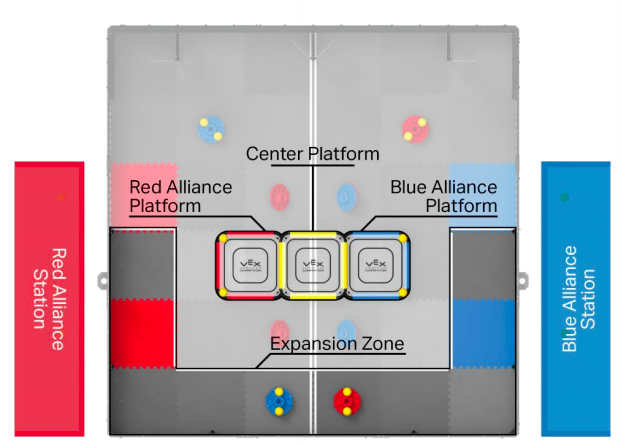
\includegraphics[height=265pt,width=\linewidth,keepaspectratio]{field/expansion } \caption{The Expansion Zone} \label{fig:expansionzone} \end{figure} 

$<SG2>$ states that \begin{quotation} 

	Once the Match begins, a Robot which is contacting the Expansion Zone may expand vertically with no height limit.
	However, once fully outside of the Expansion Zone (i.e. no longer contacting it), the Robot must return to a height limit of \inch{18} (45.72 mm) tall.
\end{quotation}

As a consequence of $<SG2>$, the robot cannot legally touch High Flags, meaning that High Flags can only be flipped using balls thrown or shot from the robot.
If the robot is to flip these High Flags, it must include capability for collecting and launching balls.
It may be helpful to examine which designs were effective in the VEX IQ “Bankshot” and VRC “Nothing But Net” challenges.

\section{Possession Limits}

$<SG4>$ states that

\begin{quote}
	Robots may Possess a maximum of one (1) Cap and two (2) Balls at a time.
\end{quote}

This means that if a robot canot employ a hoarding stratagy.
However hoarding is already banned by $<SG5>$ \par 

The more signifigan impact of $<SG4>$ will be on the design of ball launching systems, as they will have to 

\begin{itemize} \item be small enough to not have enought space for 3 balls.
	\item have the driver not pick up 3 balls.
	\item have the software moniter the number of balls in the robot
	      and automaticly shut off the ball intake once there are 2 balls
\end{itemize}

\section{Autonomous Limits}

\begin{figure}[h]
	\centering

	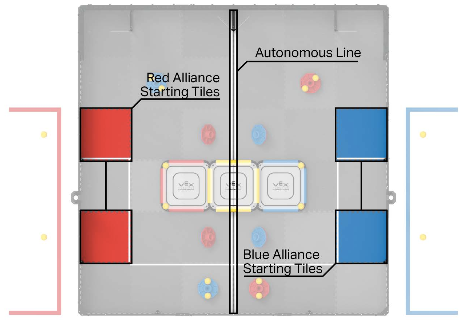
\includegraphics[height=265pt,width=\linewidth,keepaspectratio]{field/autoline}
	\caption{The Autonomous Line}
	\label{fig:autoline}
\end{figure}

By $<SG3>$, the robot may only venture into its own half of the field during the autonomous period, and no robots can centre park during this time.
	[Figure
		\ref{fig:autoline}]
\par

This means robots can be more confident in their autonamus as no enemy robots
will be on their
side

\end{document}
